% CVPR 2023 Paper Template
% based on the CVPR template provided by Ming-Ming Cheng (https://github.com/MCG-NKU/CVPR_Template)
% modified and extended by Stefan Roth (stefan.roth@NOSPAMtu-darmstadt.de)

\documentclass[12pt, oneside, a4paper]{book}
\usepackage[pagenumbers]{cvpr} % To force page numbers, e.g. for an arXiv version
\setcounter{secnumdepth}{3}
\setlength{\textheight}{8in}
\setlength{\hoffset}{0.2in}
\setlength{\textwidth}{6in}
\setlength{\headsep}{0.5in}
\setlength{\oddsidemargin}{0in}
\setlength{\evensidemargin}{0in}

%%%%%%%%% PAPER TYPE  - PLEASE UPDATE FOR FINAL VERSION

% Include other packages here, before hyperref.
\usepackage{graphicx}
\usepackage{amsmath}
\usepackage{amssymb}
\usepackage{booktabs}
\usepackage{epsf}
\usepackage{subcaption}
\usepackage{placeins}
\usepackage{paralist}
\usepackage{newtxtext, newtxmath}
\usepackage{setspace}
% It is strongly recommended to use hyperref, especially for the review version.
% hyperref with option pagebackref eases the reviewers' job.
% Please disable hyperref *only* if you encounter grave issues, e.g. with the
% file validation for the camera-ready version.
%
% If you comment hyperref and then uncomment it, you should delete
% ReviewTempalte.aux before re-running LaTeX.
% (Or just hit 'q' on the first LaTeX run, let it finish, and you
%  should be clear).
\usepackage[pagebackref,breaklinks,colorlinks]{hyperref}


% Support for easy cross-referencing
\usepackage[capitalize]{cleveref}
\crefname{section}{Sec.}{Secs.}
\Crefname{section}{Section}{Sections}
\Crefname{table}{Table}{Tables}
\crefname{table}{Tab.}{Tabs.}


%%%%%%%%% PAPER ID  - PLEASE UPDATE
\def\cvprPaperID{*****} % *** Enter the CVPR Paper ID here
\def\confName{CVPR}
\def\confYear{2023}


\onehalfspacing

\begin{document}
\pagenumbering{gobble}

%%%%%%%%% TITLE
%------------------------------------------------------------------------
% title
\title{PETIT-GAN: Physically Enhanced Thermal Images Translation Generative Adversarial Network}	
% author 
% (In the mandatory argument "{}", separate multiple
% authors with "\and" - use "\\" for better author name formatting
% in the title page. In the optional argument "[]" include all
% author names, with no "\and" or text formatting macros.)
% Example: 
%\author[A. Author Albert Einstein]{Anthony Author \and Albert Einstein}
\author[Omri Berman Dr. Iftach Klapp Navot Oz]{Omri Berman \\[.2cm]{\scriptsize Navot Oz \qquad Prof. David Mendlovic \qquad Dr. Iftach Klapp}}
% Address
%  \subtitle{\textsc{Subtitle}}

% \institute{\textsc{Volcani Center} \\
%       Optical Sensing Lab \\
%       [5pt]{\includegraphics[height=3cm,keepaspectratio]{\fulllogovolcani}}
% }
% \institute{\textsc{Tel Aviv University} \\
%       Faculty of Engineering \\
%       [5pt]{\includegraphics[height=3cm,keepaspectratio]{\logotlv}}
% }
\institute{{\includegraphics[height=2cm,keepaspectratio]{\logotlv}}
        \hfill
        {\includegraphics[height=2cm,keepaspectratio]{\fulllogovolcani}}
}

% date
\presentationDate{March 15, 2023}

\begin{frame}[plain]
    \titlepage
\end{frame}
  
{   
    \noindent
    \textbf{The results shown in this thesis have been published in the IEEE/CVF Winter Conference on Applications of Computer Vision (WACV) 2024.}
}

This work has been supported by the Israeli ministry of science and technology, research number 3-17381.

%%%%%%%%% BODY TEXT
%------------------------------------------------------------------------
\cleardoublepage
\pagenumbering{Roman}
\begin{abstract}
Thermal multispectral imagery is imperative for a plethora of environmental applications.
Unfortunately, there are no publicly-available datasets of thermal multispectral images with a high spatial resolution that would enable the development of algorithms and systems in this field.
However, image-to-image (I2I) translation could be used to artificially synthesize such data by transforming largely-available datasets of other visual modalities.
In most cases, pairs of content-wise-aligned input-target images are not available, making it harder to train and converge to a satisfying solution.
Nevertheless, some data domains, and particularly the thermal domain, have unique properties that tie the input to the output that could help mitigate those weaknesses.
We propose PETIT-GAN, a physically enhanced thermal image-translating generative adversarial network to transform between different thermal modalities - a step toward synthesizing a complete thermal multispectral dataset.
Our novel approach embeds physically modeled prior information in an UI2I translation to produce outputs with greater fidelity to the target modality.
We further show that our solution outperforms the current state-of-the-art architectures at thermal UI2I translation by approximately $50\%$ with respect to the standard perceptual metrics, and enjoys a more robust training procedure.
The code and data used for the development and analysis of our method are publicly available and can be accessed through our project's website: \href{https://bermanz.github.io/PETIT}{https://bermanz.github.io/PETIT}
\end{abstract}

{
    \hypersetup{linkcolor=black}
    \tableofcontents
    \cleardoublepage
    \listoftables
    \cleardoublepage
    \listoffigures
    \cleardoublepage
}

\pagenumbering{arabic}
\chapter{Introduction}
\label{sec:introduction}

The emergence of nanosatellites has revolutionized the field of remote sensing, allowing to acquire ground images with higher spatial resolution and at lower costs.
Many sensing systems involving nanosatellites are focused at the visible and near infrared spectrum (between 380-1400 nm) - MISC \cite{kalman2008misc} (between 380-700), Charybdis \cite{lowe2012charybdis} (between 412-870 nm) and SuperDOVE \cite{tu2022radiometric} (between 431-885 nm) to name a few.
However, very little to no attention was given to the longwave-infrared (LWIR) spectrum (7000 - 14000 nm), \aka, the thermal spectrum, which plays a crucial role in various environmental aspects, such as climate and water monitoring, fires prediction, \etc.
Identifying such phenomena requires thermal multispectral imaging, \ie, a collection of several image layers of the same scene where each layer is acquired at a particular wavelength band belonging to the thermal spectrum.
Unfortunately, while panchromatic (wide-band) thermal images were relatively easy to obtain, no off-the-shelf high-resolution thermal multispectral images were available to develop proofs of concepts for those applications.
To tackle this deficiency, we used a light-plane, a thermal camera and a set of infrared bandpass filters to collect and assemble an aerial thermal multispectral images dataset.
Due to inherent setup limitations, the amount of collected images per spectral channel was limited.
Moreover, images of different wavelengths were not spatially registered, which is essential for a complete multispectral dataset.
To overcome both the sample size and registration issues, we developed an unpaired image to image translation algorithm to transform the relatively abundant panchromatic images into pixel-wise-aligned multispectral images.

Image to image (I2I) translation is the task of transforming the style of an image to that of a different domain while preserving its content.
Many methods have been developed to tackle this task, utilizing various deep neural architectures such as auto-encoders \cite{zhao2021unpaired}, generative adversarial networks (GANs) \cite{CycleGAN2017, park2020cut, zhao2020unpaired}, diffusion models \cite{DBLP:journals/corr/abs-2104-05358, saharia2022palette} and more.
Those methods have countless applications and are being used for numerous purposes, such as synthetic dataset generation for learning tasks in fields such as autonomous cars \cite{https://doi.org/10.48550/arxiv.1812.01710, Dundar2018DomainSA}, medical imaging \cite{Thambawita_2022, chen2021synthetic}, \etc.
In most cases, as in our problem, there are no pairs of content-equivalent images in the input and output domains.
The I2I transformation in those cases is termed \emph{unpaired}.
As the unpaired image-to-image (UI2I) translation task is unsupervised and highly ill-posed, those models are usually very hard to train.

In contrast to other visual domains, thermal imaging has unique underlying physical properties that are shared across all thermal modalities.
These properties enable the design of closed-form transformations between panchromatic and multispectral images. 
In turn, those transformations can be embedded in deep UI2I architectures to improve their statistical performance and robustness.

To test this novel hypothesis, we first train two different state-of-the-art (SOTA) GANs to perform thermal UI2I translation to establish a baseline.
We then provide the generators with an additional physical property of the acquired images, allowing the GANs generator's output to be conditioned on that property.
Finally, we design a physical estimator and fuse it with the generator, resulting in our proposed method, named a physically enhanced thermal image-translating (PETIT) GAN.

Statistical analysis showed that our solution achieves an improvement of approximately $50\%$ compared to the SOTA GANs \wrt the conventional evaluation metrics.
Furthermore, our method exhibits a more robust training procedure, possibly indicating convergence to flatter minima.
These improvements are further demonstrated qualitatively through our method's greater visual fidelity to the desired target domain.

Our paper's contribution is three-fold:
(1) Application of UI2I between different thermal image modalities;
(2) Development and utilization of an analytic-physical-UI2I translation model;
(3) Introduction of a novel thermal aerial images dataset with unpaired images of different spectral bands.

\chapter{Literature review}
\label{sec:literature_review}
\section{Artificial neural network (ANN)} \label{sec:ANN}
\subsection{Background}
Artificial neural network (ANN) is a form of a nonlinear function approximator, belonging to the class of data-driven models (\aka machine learning).
The feedformward ANN architecture was originally made of multilayer perceptron (MLP), \ie, multiple layers of fully-connected perceptrons \cite{rosenblatt1957perceptron}, as schematically depicted in Figure \ref{fig:fully_connected}.
\begin{figure}[H]
    \centering
    \includegraphics[width=0.6\linewidth]{../figs/related_work/fully_connected.jpeg}
    \caption{Schematics of a MLP ANN with 2 hidden layers \cite{dabbura_2022}.}
    \label{fig:fully_connected}
\end{figure}

While the ANN has evolved significantly since its first appearance in the sixties of the previous century, the same basic principles are still being used to train all its differnet variants:
\begin{enumerate}
    \item The network takes a sample of data as an input.
    \item The data is fed forward through the network's layers to eventually produce the network's output.
    \item A loss function is used to a evaluate a property of the output that is intended to be minimized.
    \item Backpropagation (an efficient algorithm for applying the chainrule of derivation) is used to calculate the loss function's partial derivatives \wrt the ANN's parameters (\aka weights).
    \item The stochastic gradient decent algorithm \cite{cauchy1847methode} uses the gradient vector of partial derivatives to  update the ANN's weights to minimize the loss function.
    \item Steps 1-5 are being repeated iteratively across different data samples and their permutations until some predefined stopping criteria is met.
\end{enumerate}

Along the years, ANNs continued to evolve in several aspects (\eg the adoption of cross-entropy loss, rectified linear units (ReLU) \cite{nair2010rectified}, \etc), but, until recently, remained somewhat unpopular compared to other machine learning methods.
In 2012, \emph{AlexNet} \cite{10.5555/2999134.2999257} an ANN achieved the best top-5 classification score on ImageNet \cite{5206848} classification contest.
Ever since, ANNs and their configurations have grown widely popular and became the SOTA solutions to a variety of real world problems in the fields of natural language processing (NLP), computer vision (CV) and many more.

\subsection{Convolutional neural network (CNN)}
In addition to the growing amount of applications to which ANNs made significant contributions, great progress was also made in the field of ANN architectures.
Among the significant advances were CNNs \cite{lecun1995convolutional}, which are built of layers of two-dimensional convolution kernels rather than perceptrons.
Convolutions are especially helpful when working with visual data, as they leverage the spatial correlation between neighboring pixels, allowing to identifying meaningful local features.
CNNs are also typically more computationally efficient, as they are made of sparse interactions between two adjacent layers \cite{Goodfellow-et-al-2016},rather than being fully-connected, and allow working with data of variable spatial dimensions.
A convolutional layer of a CNN is typically made up of 3 components:
\begin{enumerate}
    \item Convolutions: Different kernels of convolution. Their size affect the receptive field and their amount define the depth of the layer's output feature map.
    \item Normalization: A form of normalizing the layer's input to improve stability and regularity, either batchwise (\aka BatchNorm \cite{DBLP:journals/corr/IoffeS15}), per-instance (\aka InstanceNorm \cite{ulyanov2016instance}) or none at all.
    \item Activation: A non-linear function that's applied elementwise over the normalized convolution output. 
    These layers are the crucial component in allowing deep neural network to approximate extremely complex and highly-nonlinear target functions.
    Without activations, neural networks are essentially equivalent to a single linear layer, making them no more capacitated than a simple linear predictor.
    Among the common activation functions are sigmoids, hyperbolic tangent, and the ReLU discussed in the previous subsection.
    \item Pooling: A function that summarizes some statistics of neighborhoods of elements in some feature map (\eg, the average within a $2 \times 2$ rectangle neighborhood of pixels).
    Pooling results in a single scalar per neighborhood of elements, further distilling the knowledge obtained by the convolution and reducing the spatial size of its latent feature maps.
    One of the most common pooling statistics is the max-pooling \cite{Zhou1988ComputationOO}, which picks the maximum element from within each neighborhood.
\end{enumerate}

\subsection{Residual blocks}
Due to their typical structure, the more complex and nonlinear the approximated function is - the deeper the ANNs should get (there are some exceptions to that claim, but it is generally true).
However, increasing the number of layers of an ANN means that the gradients have longer paths to travel during backpropagation.
When a network becomes very deep, it typically suffers from either \emph{vanishing gradients} or \emph{vanishing gradients} \cite{bengio2013advances}, phenomena related to issues with the gradients' norms.
In 2015, He \etal \cite{DBLP:journals/corr/HeZRS15} delveloped the concept of residual blocks (\emph{ResBlocks}), where each layer of the network acted as a residual function \wrt its input layer.
ResBlocks are essentially made up of two consequent weight layers (either a fully connected or a convolutional layer) with a ReLU activation in between, followed by a summation of the ResBlock's output and input (\aka skip-connection), and finally one additional ReLU activation over the result.
A schematic depiction of a residual block can be seen in Figure \ref{fig:ResBlock}.
\begin{figure}[H]
    \centering
    \includegraphics[width=0.7\linewidth]{../figs/related_work/residual_block.png}
    \caption{The architecture of a residual block \cite{He2016DeepRL}.} 
    \label{fig:ResBlock}
\end{figure}
By concatenating several ResBlocks together (\emph{ResNet}), He \etal managed to beat previous SOTA methods over ImageNet classification by a large margin. For the first time, it was possible to train ANNs with hundreds of layers, enabling approximation of functions with growing complexity and nonlinearity.

\subsection{Computer vision}
As mentioned before, ANNs play a significant role in the field of computer vision, and are the basis for SOTA solutions in various CV tasks.
Among the most popular CV tasks carried by ANNs are:
\begin{enumerate}
    \item Binary classification: Classifying images between two types of classes, \eg, Kaggle's dogs \vs cats challenge.
    \item Multi-class classification: Classying images between several different classes, \eg, ImageNet classification challenge where there are 1000 different classes.
    \item Semantic segmentation: Producing a per-pixel classification map rather than assigning a single label for the entire image.
    \item Object detection: Identifying a region in the image where some object appears, \eg, detecting a human face in an image. 
    Typically, the output of a detection algorithm is a rectangular bounding-box enclosing the detected object.
\end{enumerate}

One CV task of growing popularity is that of artificial data generation.
While most CV tasks take an input and produce some form of distilled information, data generation takes some input (and sometimes no input at all) and hallucinates new data.
In the domain of ANNs, there are five popular architectures that are typically used for data generation tasks:
\begin{enumerate}
    \item Variational auto-encoder (VAE) \cite{kingma2013auto}: an encoder and a decoder (essentially 2 ANNs) are trained jointly to simultaneously reconstruct an input image and minimize the Kullback-Leibler divergence \cite{csiszar1975divergence} between the distribution of the input's embedding, \ie, the feature map obtained by forward-passing the input through several hidden layers, and a normal distribution. 
    These models are usually designed to hallucinate interpolations between images belonging to the input domain rather than for transforming data to a different modality.
    \item Generative adversarial network (GAN) \cite{goodfellow2014generative}: A generator and a discriminator (again, two separate ANNs) are trained alternately with adversarial objectives. 
    The generator hallucinates an image from the target distribution that's suppose to fool the discriminator, while the discriminator attempts to classify between real images and ones that were created by the generator.
    An extensive overview about generative models will appear in the following subsection.
    \item Vision transformer (VIT) \cite{dosovitskiy2020image}: Inspired by natural language processing transformers and the attention mechanism \cite{vaswani2017attention}, VITs use both the global and local context of an input image to solve the task at hand.
    Data generation is only one of many different CV tasks tackled by VITs.
    In the region of large amounts of data, transformers are considered to outperform their counterparts.
    \item Normalizing flows \cite{rezende2015variational}: instead of implicitly training the network to transform a random sample from some probability distribution to a sample from the target domain, normalizing flows go the other way around, \ie, learn to transform the target domain to a predefined probability distribution.
    Normalizing flows utilize bijective functions as building blocks, such that the obtained transformation is invertible.
    At inference time, the inverse transformation is applied to transform a sample from the regular probability distribution to the target domain.
    \item Diffusion models\cite{sohl2015deep}: avoiding the need for a discriminator/critic, diffusion models aim to transform the prior target data distribution into random noise before revising the transformations step by step so as to rebuild a brand new sample with the same distribution as the prior.
    By some criteria, diffusion models are considered to beat GANs at generative tasks, \eg, in the work of Dhariwal \etal \cite{dhariwal2021diffusion}, where a diffusion model exhibit improved unconditional image generation results compared to SOTA GANs.

\end{enumerate}


\section{Generative adversarial newtwork}
GAN is a class of deep generative models, first introduced by Goodfellow \etal \cite{goodfellow2014generative}.
Images are the most common product of GANs, but there is no restriction in using them to produce other types of data as well.

\subsection{Architecture}
As explained in section \ref{sec:ANN}, GANs are made of a generator and a discriminator that are trained adversarially, (hopefully) until convergence.

The generator is an ANN that typically samples a random vector from some predefined probability density function, commonly Gaussian or uniform, and transforms it into an output whose dimensions match the target domain.
At initialization, the generator has no sense of the expected outcome of its transformation, and thus, assuming its weights are randomly initialized, produces a purely arbitrary output.
As training progresses, given that the discriminator generates a viable feedback, the generator adjusts its transformation to result in more authentic outputs.
The ultimate target of the generator is to fool the discriminator, \ie, to produce outputs that are indistinguishable from real data belonging to the target domain, in the "eyes" of the discriminator.

The discriminator (\aka critic in some contexts) is also an ANN, whose purpose is to discriminate between real images from the target domain and images forged by the generator.
Every sample observed by the discriminator is tagged along with a ground truth label indicating whether the image is actually real or fake (artificially generated).
    
Clearly, the better performing the generator is, the more difficult the classification task of the discriminator becomes.
Accordingly, the better the discriminator is at classifying between real and fake images, the more difficult it is for the generator to hallucinate outputs that would fool the discriminator.
This entangled setup is the reason GAN's training procedure is referred to as adversarial.
The schematics of a typical GAN are depicted in Figure \ref{fig:gan_arch}.
\begin{figure}[H]
    \centering
    \includegraphics[width=\linewidth]{../figs/related_work/gan_arch.png}
    \caption{Schematics of a typical GAN for generating human-like faces \cite{radhakrishna_2020}.}
    \label{fig:gan_arch}
\end{figure}

\subsection{Loss function}
In the original paper, the GAN's adversarial objective function is the following:
\begin{equation} \label{eq:origGanLoss}
    \mathcal{L}(D,G) = \underset{x}{\mathbb{E}}\left[log\left(D(x)\right)\right] + \underset{z}{\mathbb{E}}\left[log\left(1 - D\left(G(z)\right)\right)\right]
\end{equation}
Where $x$ are real images from the target domain, $z$ are random vectors drawn from some predefined probability density function, $D(\cdot)$ is the discriminator's activation function (sigmoid), and $G(\cdot)$ is the generator's output.
While the discriminator attempts to maximize the objective, the generator tries to minimize it, resulting in a minimax adversarial setting ($\underset{G}{min}\underset{D}{max} \mathcal{L}(D,G)$).

In practice, it is not feasible to train both the generator and the discriminator simultaneously, as ones loss depends on the other's intrinsic parameters.
Therefore, at every iteration, one's weights are frozen while the other incurs its loss and updates its weights accordingly.
As this is the case, the generator's loss objective can be reduced to a single term:
\begin{equation}\label{eq:GanLossOnly}
    \underset{G}{min} \mathbb{E} \left[log\left(1 - D\left(G(z)\right)\right)\right]
\end{equation}
As noticed by the authers of the original paper, the loss in equation \ref{eq:GanLossOnly} tends to saturate. 
To avoid that, instead of minimizing the probability of fake classification, they proposed to instead maximize the probability of real classification:
\begin{equation}
    \underset{G}{max} \mathbb{E} \left[log\left(D\left(G(z)\right)\right)\right]
\end{equation}

While successful in several tasks, the discriminator's cross-entropy loss often results in the vanishing gradient problem described in the section \ref{sec:ANN}.
To overcome it, Mao \etal \cite{mao2017least} introduced LSGAN (Least Squares GAN) where squared error (\aka $\ell_2$ loss) is used for the discriminator's loss instead of sigmoid.
LSGAN significantly improved the generated data's quality, as well as the training stability.
More recently, Arjovsky \etal \cite{arjovsky2017wasserstein} proposed WGAN, where the earth mover (EM) distance is utilized as a loss function instead of cross-entropy or $\ell_2$.
This method assumes a 1-Lipschitzness over both generator and discriminator (sometimes enforced by gradient clipping) and is said to significantly improve stability and mitigate the notorious mode-collapse phenomenon.
Many more types of improvements to the GANs loss function were suggested along the years, but those described above were the most famous and popular ones.

\subsection{Types and applications}
Since the original GAN paper, a great deal of different types of GANs were developed for many different purposes.
Many of those developments form the underlying principles and architecture of numerous state-of-the-art models of several applications, and are way too many to cover in this mass.

Among the various tasks performed by GANs is I2I translation, where the output is conditioned on an input image.
I2I translation has a plethora of applications, such as image segmentation \cite{yang2018mri, li2020simplified}, pose estimation \cite{li2020manigan, fish2017adversarial}, colorization \cite{isola2017image, suarez2017infrared, zhang2017real}, super resolution \cite{yuan2018unsupervised, zhang2019multiple} and many more.
The I2I translation task can be roughly classified into two classes:
\begin{enumerate}
    \item Supervised / paired I2I ( I2I), where each image in the input domain has a content-aligned equivalent in the output domain. 
    \item Unsupervised / unpaired I2I (UI2I), where there are no content-equivalent pairs in the input and output domains.
\end{enumerate}
Most practical I2I tasks are performed in an unsupervised fashion, as fully registered pairs of images in two different modalities are extremely difficult to obtain.
An example of a paired \vs unpaired I2I training examples is given in Figure \ref{fig:paired_vs_unpaired}.
\begin{figure}[H]
    \centering
    \includegraphics[width=0.75\linewidth]{../figs/related_work/paird_vs_unpaired_I2I.png}
    \caption{Paired I2I samples of sketch-to-image translation (left) \vs unpaired I2I samples of image-to-painting translation (right) \cite{CycleGAN2017}.}
    \label{fig:paired_vs_unpaired}
\end{figure}
    
The great challenge in UI2I translation is that no ground truth is available as a reference for the transformed output.
Thus, in contrast to paired I2I, pixel-level loss cannot be used to steer the training toward a better content-preserving solution.
Therefore, content preservation of the transformation must be enforced by an alternative mechanism.
The most popular strategy to ensure content preservation is to use cycle consistency \cite{Lee_2018_ECCV}.
This approach relies on two translators: one from domain A to domain B ($G_{A \rightarrow B}$), and one in the opposite direction ($G_{B \rightarrow A}$). 
Additive to the standard adversarial loss, cycle-consistency is used to penalize for discrepancies between input $x_A$ and its reconstruction by the roundtrip transformation from A to B and then back to A:
\begin{equation}
    \mathcal{L}_{cyc} = \mathcal{L}\left( x_A, G_{B \rightarrow A} \left( G_{A \rightarrow B}(x_A) \right) \right)
\end{equation}
CycleGAN \cite{CycleGAN2017}, along with DiscoGAN \cite{kim2017learning} and DualGAN \cite{yi2017dualgan} additionally impose cycle consistency over images originating in domain B, resulting in two simultaneous cyclic losses.

More cyclic-loss based extensions were suggested along the years, proposing to use a shared latent space between input and output \cite{liu2017unsupervised}, incorporating an attention module for regions of interest \cite{kim2019u} and many more.

While successfully eliminating the need for ground truth, cycle consistency inherently encourages the transformation to encode information about the input that serves solely for the purpose of cyclic reconstruction.
This encoded information comes at the expense of fidelity to the target modality, which is clearly undesirable.
In an attempt to eliminate the need for cycle consistency, several approaches have implemented a one-sided translation that manages to preserve content in a different fashion.
Typically, this is done by embedding both input and target in some shared style-agnostic space. 
The geometric distance between the embeddings is treated as a measure of content discrepancy, and then minimized to improve content preservation.
Fu \etal \cite{fu2019geometry} encouraged preservation of the geometric relationship between an input and its geometrically transformed versions and their outputs. 
Both F-LSeSim \cite{zheng2021spatially} and contrastive unpaired translation (CUT) \cite{park2020cut} used contrastive representation learning by maximizing the similarity between pairs of corresponding patches in the input and output, and minimizing it for non-matching patches.

In this thesis, we built upon the architectures of both CycleGAN and CUT.
Therefore, we provide some further attention to those model and describe them in more detail.

\subsubsection{CycleGAN}
As explained, CycleGAN \cite{CycleGAN2017} is a cycle-consistency-loss-based GAN for performing UI2I.
CycleGAN was among the first models and probably one of the most famous architectures for performing UI2I.
The loss function of CycleGAN is a weighted sum of different components:
\begin{itemize}
    \item adversarial loss (specifically, patch LSGAN loss, which calculates the least-squared GAN loss for random patches).
    \item Cycle-consistency loss, for each of A and B data domains, between an input and its reconstructed version. The authors used $\ell_1$ distance as the discrepancy measure. put in math:
    \begin{equation}
        \mathcal{L}\left( x_A, G_{B \rightarrow A} \left( G_{A \rightarrow B}(x_A) \right) \right) = 
        ||x_A - G_{B \rightarrow A} \left( G_{A \rightarrow B}(x_A) \right)||_1
    \end{equation}
    \item Identity loss, where an input of domain A is transformed by $G_{B \rightarrow A}$, as if it was an image from domain B, and compared to the original input.
    The idea behind identity loss is to minimize the effect that the generator $G_{B \rightarrow A}$ has on images from domain $A$.
    This helps mitigate color discrepancy issues that otherwise arise when applying the cycle transformation.
    The $\ell_1$ was used for the identity loss as well.
\end{itemize}
In each training iteration, the weighted loss is evaluated simultaneously for input batches from domain A and from domain B.
The schematics of the CycleGAN architecture is depicted in Figure \ref{fig:CycleGAN_loss_schematics}.
\begin{figure}[H]
    \centering
    \includegraphics[width=0.8\linewidth]{../figs/related_work/CycleGAN_arch.png}
    \caption{Schematic of the CycleGAN's architecture \cite{chandhok_2022}.}
    \label{fig:CycleGAN_loss_schematics}
\end{figure}

CycleGAN was trained and utilized for several different purposes, such as horses $\rightarrow$ zebras, winter $\rightarrow$ summer, apples $\rightarrow$ oranges, \etc.
Exemplary results of the these trained translations can be observed in Figure \ref{fig:CycleGAN_results}.
\begin{figure}[H]
    \centering
    \includegraphics[width=0.3\linewidth]{../figs/related_work/CycleGAN_results.png}
    \caption{CycleGAN's exemplary results for different UI2I tasks \cite{CycleGAN2017}.}
    \label{fig:CycleGAN_results}
\end{figure}

\subsubsection{CUT}
Contrastive unpaired translation (CUT) GAN \cite{park2020cut} belongs to the family of non-cycle-consistent models for UI2I.
Many of CUT's design choices match those of CycleGAN variants (\eg, using 9 ResBlocks as the generator's backbone).
To handle the lack of cycle-consistency, an alternative patchwise contrastive loss is applied instead.
The procedure for calculating the contrastive loss is as follows:
\begin{enumerate}
    \item An input image $x$ of some domain is translated via a generator to a different domain(same as in CycleGAN):
    \begin{equation*}
        y = G(x)        
    \end{equation*}
    \item Random non-overlapping patches of the input $x$ and output $y$ are selected correspondingly, \ie, each patch of $x$ spatially corresponds to a patch in $y$.
    \item The random patches of both $x$ and $y$ are fed into the same generator ($G(\cdot)$), and prominent latent feature maps are concatenated to assemble a feature tensors $\tilde{x}$ and $\tilde{y}$.
    \item A multilayer perceptron (MLP) network is used to encode all the feature tensors into vectors in a dedicated embedding space.
    \item Cross-entropy loss is used to encourage similarity between spatially corresponding patches in $\tilde{x}$ and $\tilde{y}$, and minimize that similarity between non-corresponding patches.
    This is the contrastive loss that guarantees spatial coherency between the input and target domains, as it constraints that the generator maintains a high mutual information between activations of its input and output.
\end{enumerate}
An illustration of the patchwise contrastive loss calculation process appears in Figure \ref{fig:CUT_contrastive_sceheme}.
\begin{figure}[H]
    \centering
    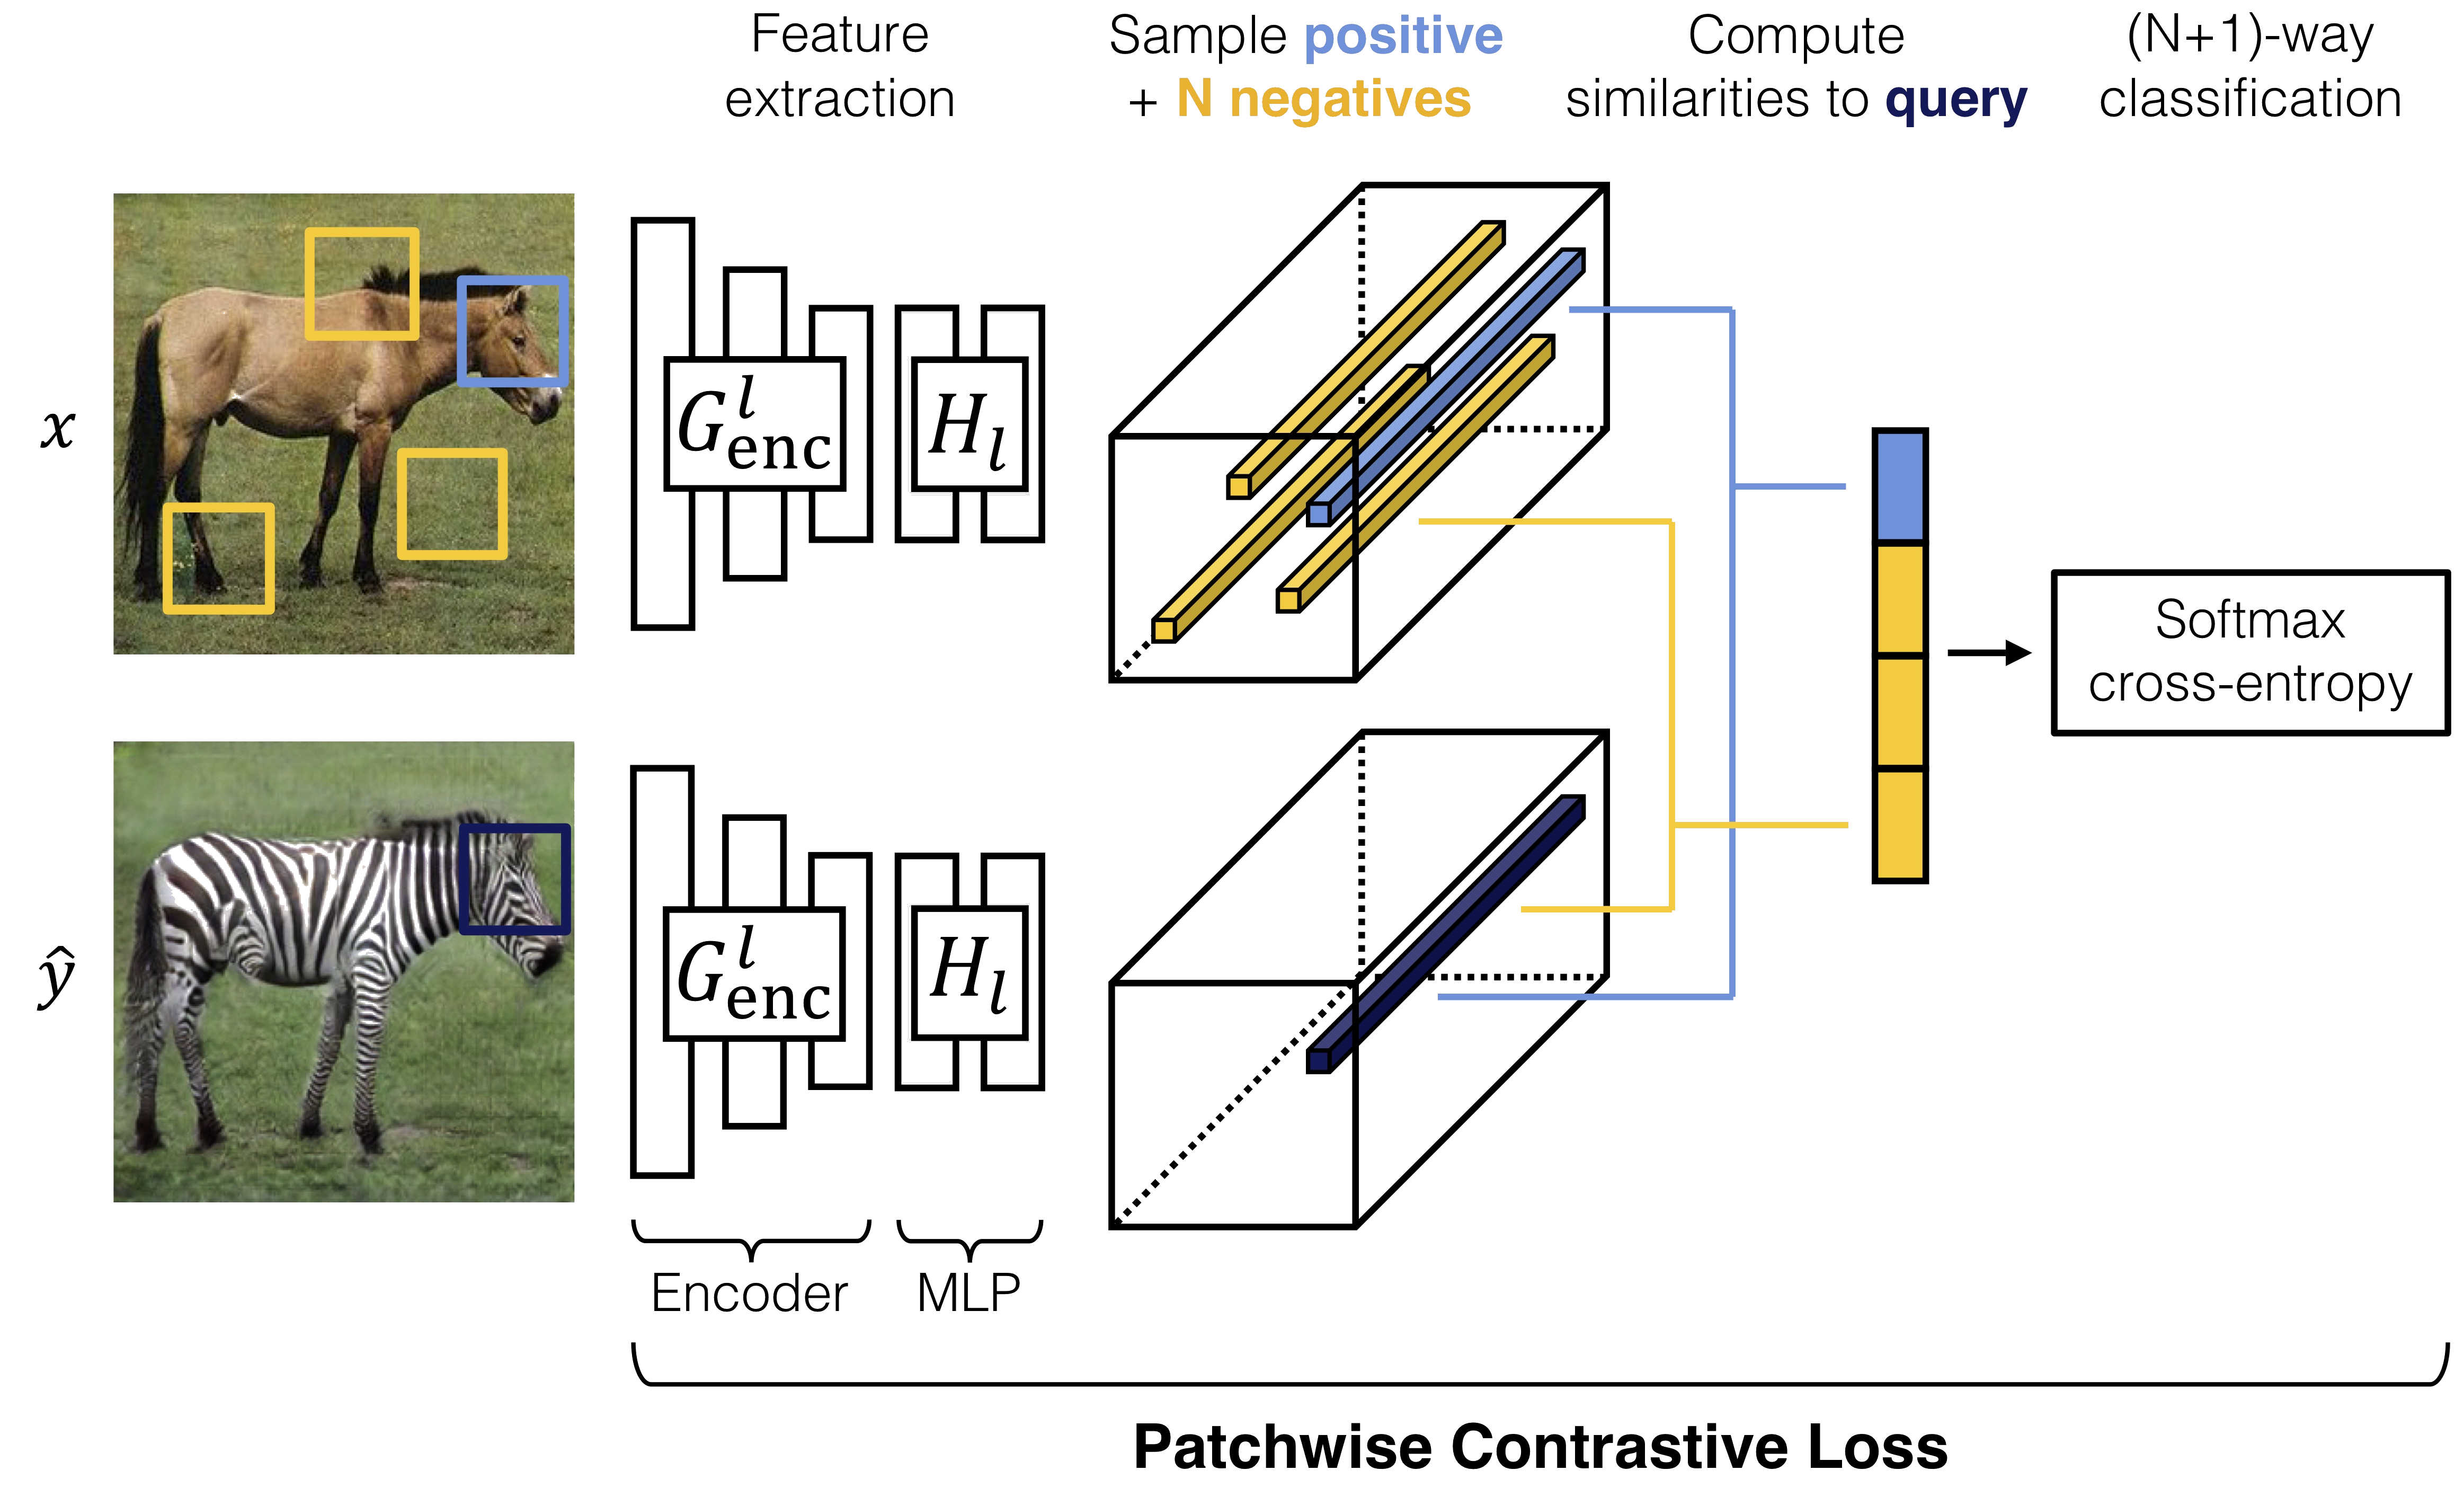
\includegraphics[width=\linewidth]{../figs/related_work/CUT_contrastive_sceheme.jpg}
    \caption{Schematic of the patchwise contrastive loss calculation procedure \cite{park2020cut}.}
    \label{fig:CUT_contrastive_sceheme}
\end{figure}    

The other loss components, \ie, adversarial loss and identity loss, were the same as in CycleGAN.
As claimed by the authors, the elimination of the second set of generator and discriminator and the cyclic reconstruction resulted in a more stable and memory efficient solution, which produces superior results to that of CycleGAN.

\section{Thermal imaging}

\subsection{Blackbody radiation}
Black-body radiation is the thermal electro-magnetic signal that is emitted by an ideal opaque object due to its temperature.
Planck's law of black-body radiation states that:
\begin{equation} \label{eq:Plancks-law}
  B_{\lambda}(T) = \frac{2\pi hc^2}{\lambda^5}\frac{1}{e^{\frac{hc}{\lambda kT}} - 1} \; \; \left[W sr^{-1} m^{-2} \mu m^{-1}\right]
\end{equation}
where $B_{\lambda}(T)$ is the ideal object's spectral radiance density, $h$ is Planck's constant, $c$ is the speed of light in a vacuum, $k$ is the Boltzmann constant, $\lambda$ is the electromagnetic wavelength and $T$ is the object's absolute temperature \cite{FundamentalsOfInfraredThermalImaging}.
As evident from Planck's law, the spectral radiance density is different depending on the object's temperature, as depicted in Figure \ref{fig:Planck_density}.
\begin{figure}[H]
  \centering
  \includegraphics[width=\linewidth]{../figs/methods/planck.png}
  \caption{Planck's spectral radiance densities for different object temperatures \cite{enwiki:1128338285}.}
  \label{fig:Planck_density}
\end{figure}

The Stefan-Boltzmann law \cite{surhone2010stefan} ties the power radiated from an object (which is the result of integrating $B_{\lambda}(T)$ over the entire spectrum of wavelengths from zero to infinity) to the object's temperature:
\begin{equation} \label{eq:stephan-boltzmann-ideal}
    P(T) = \int_0^\infty B_{\lambda}(T) d\lambda = \frac{\sigma}{\pi} T^4 \; \;\left[W sr^{-1} m^{-2}\right]
\end{equation}
where $P$ is the radiated power and $\sigma$ is the Stephan-Boltzmann constant. 

A real-world opaque object emits less power than an ideal black body at the same temperature. 
The ratio between the radiation emission of an object and that of an ideal blackbody at the same temperature is called \emph{emissivity}.
The emissivity is a function of various a-priori unpredictable characteristics of the object, such as material type, surface structure, viewing angle, \etc.
Thus, the Stephan-Boltzmann law for practical objects is given by:
\begin{equation} \label{stephan-boltzmann-practical}
  P(T) =  \frac{\sigma}{\pi} \epsilon T^4 \; \; \left[W sr^{-1} m^{-2}\right]
\end{equation} 
where $\epsilon$ is the object's emissivity.
In general, the emissivity is a function of the wavelength \cite{kerekes2008spectral}, but it is used here as a constant that reflects its expected value over the thermal bandwidth for simplification.

\subsection{Microbolometric camera acquisition}
Microbolometric camera is a thermal camera who's sensor is a microbolometer, which is a thermally sensitive resistor.
According to \cite{FundamentalsOfInfraredThermalImaging}, when acquired by a thermal microbolometric camera with a finite bandwidth, the incident power on the microbolometer (the thermal camera's sensor) can be described by:
\begin{equation} \label{BolometerIncidentPower}
  \phi(T) = \gamma F_\mathit{pan} \epsilon T^4 \; \; \left[W sr^{-1} m^{-2}\right]
\end{equation}
where $\phi$ is the incident power on the microbolometer, $\gamma$ is a constant governed by the camera's geometrical properties and $F_\mathit{pan}$ represents the fraction of power that is within the camera's bandwidth.
When applying an IR bandpass filter over the camera lens, equation \ref{BolometerIncidentPower} still holds except that $F_\mathit{pan}$ is replaced by $F_\mathit{mono}$, reflecting the fraction of power that is strictly within the bandpass region of the applied filter \cite{FundamentalsOfInfraredThermalImaging}.

Since $\gamma, F_\mathit{pan}, \epsilon$ are all constants, they can be reduced into a single coefficient:
\begin{equation} \label{BolometerIncidentPowerSimplified}
  \phi(T) = a T^4 \; \; \left[W sr^{-1} m^{-2}\right]
\end{equation}
suggesting that the incident power is proportional to $T^4$.
Consequently, a thermally stabilized camera operating in radiometric mode, \ie, when the image intensity levels are linear in the incident power, the intensity of a pixel is obtained by an affine transformation of $T^4$:
\begin{equation} \label{eq:naiveAffineTrans}
  I(T) = b + a T^4
\end{equation}
where $I$ is the intensity level of the pixel and $b$ is the digital bias level. 


\chapter{Proposed method}
\label{sec:methods}
Toward synthesizing a multispectral dataset, we showcase the UI2I transformation between a panchromatic modality, \ie, a wide-band thermal image, and a single monochromatic modality, \ie, a narrow-band thermal image.
More concretely, we transform images with a bandwidth of $7 - 14 \mu m$ to images with a central wavelength of $9\mu m$ and a full width at half maximum (FWHM) of $0.5 \mu m$.
For ease of notation, we will use the subscripts \emph{pan} to describe panchromatic data, and \emph{mono} for monochromatic.
This concept could be easily extended to synthesize a complete multispectral dataset by applying it repeatedly for disjoint sub-bands of the thermal spectrum to full coverage.
\subsection{Physical estimator}

\subsubsection{Background}
Black-body radiation is the thermal electro-magnetic signal that is emitted by an ideal opaque object due to its temperature.
Planck's law of black-body radiation states that:
\begin{equation} \label{eq:Plancks-law}
  B_{\lambda}(T) = \frac{2\pi hc^2}{\lambda^5}\frac{1}{e^{\frac{hc}{\lambda kT}} - 1} \; \; \left[W sr^{-1} m^{-2} \mu m^{-1}\right]
\end{equation}
where $B_{\lambda}(T)$ is the ideal object's spectral radiance density, $h$ is Planck's constant, $c$ is the speed of light in a vacuum, $k$ is the Boltzmann constant, $\lambda$ is the electromagnetic wavelength and $T$ is the object's absolute temperature \cite{FundamentalsOfInfraredThermalImaging}.
The Stefan-Boltzmann law \cite{surhone2010stefan} ties the power radiated from an object (which is the result of integrating $B_{\lambda}(T)$ over the entire spectrum of wavelengths from zero to infinity) to the object's temperature:
\begin{equation} \label{eq:stephan-boltzmann-ideal}
    P(T) = \int_0^\infty B_{\lambda}(T) d\lambda = \frac{\sigma}{\pi} T^4 \; \;\left[W sr^{-1} m^{-2}\right]
\end{equation}
where $P$ is the radiated power and $\sigma$ is the Stephan-Boltzmann constant. 

A real-world opaque object emits less power than an ideal black body at the same temperature. 
The ratio between the radiation emission of an object and that of an ideal blackbody at the same temperature is called \emph{emissivity}.
The emissivity is a function of various a-priori unpredictable characteristics of the object, such as material type, surface structure, viewing angle, \etc.
Thus, the Stephan-Boltzmann law for practical objects is given by:
\begin{equation} \label{stephan-boltzmann-practical}
  P(T) =  \frac{\sigma}{\pi} \epsilon T^4 \; \; \left[W sr^{-1} m^{-2}\right]
\end{equation} 
where $\epsilon$ is the object's emissivity.
In general, the emissivity is a function of the wavelength \cite{kerekes2008spectral}, but it is used here as a constant that reflects its expected value over the thermal bandwidth for simplification.

According to \cite{FundamentalsOfInfraredThermalImaging}, when acquired by a thermal microbolometric camera with a finite bandwidth, the incident power on the microbolometer (the thermal camera's sensor) can be described by:
\begin{equation} \label{BolometerIncidentPower}
  \phi(T) = \gamma F_\mathit{pan} \epsilon T^4 \; \; \left[W sr^{-1} m^{-2}\right]
\end{equation}
where $\phi$ is the incident power on the microbolometer, $\gamma$ is a constant governed by the camera's geometrical properties and $F_\mathit{pan}$ represents the fraction of power that is within the camera's bandwidth.
When applying an IR bandpass filter over the camera lens, equation \ref{BolometerIncidentPower} still holds except that $F_\mathit{pan}$ is replaced by $F_\mathit{mono}$, reflecting the fraction of power that is strictly within the bandpass region of the applied filter \cite{FundamentalsOfInfraredThermalImaging}.

Since $\gamma, F_\mathit{pan}, \epsilon$ are all constants, they can be reduced into a single coefficient:
\begin{equation} \label{BolometerIncidentPowerSimplified}
  \phi(T) = a T^4 \; \; \left[W sr^{-1} m^{-2}\right]
\end{equation}
suggesting that the incident power is proportional to $T^4$.
Consequently, a thermally stabilized camera operating in radiometric mode, \ie, when the image intensity levels are linear in the incident power, the intensity of a pixel is obtained by an affine transformation of $T^4$:
\begin{equation} \label{eq:naiveAffineTrans}
  I(T) = b + a T^4
\end{equation}
where $I$ is the intensity level of the pixel and $b$ is the digital bias level. 

Based solely on equation \ref{eq:naiveAffineTrans}, we can seemingly infer an object's temperature directly from the thermal image intensity and vice versa.
However, when dealing with an uncooled (non-thermally stabilized) microbolometric camera, the coefficients in the equation are highly sensitive to the camera's intrinsic temperature. 
According to \cite{10.1117/1.OE.52.6.061304}, the dependency of those coefficients on the intrinsic temperature can be faithfully approximated by a third-order polynomial, concluding that a more accurate description of a pixel's intensity level is
\begin{equation} \label{IntensityVsTemperatures}
  I(T_\mathit{obj}, T_\mathit{int}) = p^{(0)}_c(T_\mathit{int}) + p^{(1)}_c(T_\mathit{int}) T^4_\mathit{obj}
\end{equation}
where $T_\mathit{obj}$ is the object's absolute temperature, $T_\mathit{int}$ is the camera's intrinsic temperature at the time of acquisition, and:
\begin{equation} \label{poly_formula}
  p^{(i)}_c(T_\mathit{int}) = \sum_{k=0}^3  c_{i,k} T_\mathit{int}^k
\end{equation}
where the superscript $^{(i)}$ indicates that the two polynomials in equation \ref{IntensityVsTemperatures} have different coefficients.
Plugging equation \ref{poly_formula} into \ref{IntensityVsTemperatures} and simplifying all of the terms gives:
\begin{equation} \label{eq:full_expr}
  \begin{split}
    I(T_\mathit{obj}, T_\mathit{int}) &= c_{0,0} + c_{0,1} \cdot T_\mathit{int} + c_{0,2} \cdot T^2_\mathit{int} \\
    & + c_{0,3} \cdot T^3_\mathit{int} + (c_{1,0} + c_{1,1} \cdot T_\mathit{int} \\
    & + c_{1,2} \cdot T^2_\mathit{int} + c_{1,3} \cdot T^3_\mathit{int}) \cdot T^4_\mathit{obj} \\
    &= <F, C>
  \end{split}
\end{equation}
where in the last transition, we factorize the relationship as an inner product by stacking all monomials in a single feature vector $F$ and all coefficients in a vector $C$.
Overall, the estimator in equation \ref{eq:full_expr} is made up of eight different monomials and parametrized by eight corresponding coefficients.

\subsubsection{Estimator modeling}
Traditionally, the coefficients from equation \ref{IntensityVsTemperatures} are calibrated to estimate an object's temperature given a measured intensity.
However, we noticed that it could also be used in the opposite direction, \ie, to produce a thermal image intensity given a known object temperature. 
Our innovation is in combining the two directions of applying equation \ref{IntensityVsTemperatures} in a cascade to assemble an analytic UI2I translation model in the following way: 

Given a set of calibrated panchromatic coefficients, we can estimate the object's temperature using the panchromatic intensity and the intrinsic temperature at acquisition:
\begin{equation} \label{eq:backward_poly}
  \hat{T}_\mathit{obj} = \sqrt[4]{\frac{I_\mathit{pan} - p^{(0)}_{c_\mathit{pan}}(T_\mathit{pan})}{p^{(1)}_{c_\mathit{pan}}(T_\mathit{pan})}}
\end{equation}
With the estimated object temperature at hand, we can invoke equation \ref{IntensityVsTemperatures} once again, this time using calibrated monochromatic coefficients, to estimate the monochromatic intensity:
\begin{equation} \label{eq:forward_poly}
  \hat{I}_\mathit{mono} = p^{(0)}_{c_\mathit{mono}}(T_\mathit{mono}) + p^{(1)}_{c_\mathit{mono}}(T_\mathit{mono}) \hat{T}_\mathit{obj}^4
\end{equation}
We treat the cascaded utilization of equations \ref{eq:backward_poly} and \ref{eq:forward_poly} as the physical estimator, and denote it by $G_{\mathit{phys}}$. Formally:
\begin{equation}
  \hat{I}_\mathit{mono} = G_{\mathit{phys}}(I_\mathit{pan}, T_\mathit{pan}, T_\mathit{mono})
\end{equation}

\subsubsection{Estimator coefficient calibration} \label{subsubsec:calibration}
Our in-house-designed calibration setup consists of a thermal camera, blackbody target (to control the scene's temperature) and an environmental chamber (to control the camera's ambient temperature).
The setup was used to capture images of varying scenes and ambient temperatures, to cover the three-dimensional $T_\mathit{int}$-$T_\mathit{obj}$-intensity space.
We then used the measurements to solve for the physical estimator's coefficients using a least-squares minimization criterion.
The calibration results of an exemplary pixel can be visualized as a surface in the three-dimensional $T_\mathit{int}$-$T_\mathit{obj}$-intensity space, as shown in Figure \ref{physical_model_fit}.
\begin{figure}
  \centering
  \includegraphics[width=\linewidth]{../figs/methods/physical_model_tight.pdf}
  \caption{An example surface fit visualizing the calibrated polynomial coefficients of a single pixel.}
  \label{physical_model_fit}
\end{figure}
Since the physical estimator requires both panchromatic and monochromatic calibrated coefficients, the calibration process was conducted twice, with and without applying an IR bandpass filter over the camera lens.
For a more elaborate description of the calibration process, please refer to section \ref{Supp-sec:calibration} in the supplementary material.

As it turns out, the calibrated physical estimator was not very accurate, and in particular suffered from a significant first-order error.
Those inaccuracies might have had to do with issues related to the calibration setup, which would normally require an exhaustive investigation to find its root cause.
To circumvent this cumbersome effort, we applied a pixel-wise affine transformation to the estimator, \ie: 
\begin{equation}
  \tilde{G}_{\mathit{phys}} = A \circ G_{\mathit{phys}} + B
\end{equation}
where $A, B$ are matrices and $\circ$ is the Hadamard product operator.
By constructing the elements of the matrices $A, B$ as learnable parameters, back-propagation can be utilized to implicitly correct the physical estimator's prediction of the monochromatic output.


\subsection{Deep estimator}
Given the calibrated physical estimator, one might wonder why this is not enough to solve the UI2I task altogether. 
Unfortunately, as evident from equation \ref{stephan-boltzmann-practical}, the emissivity can utterly change the incident thermal radiation on the camera's sensor. 
Therefore, two objects sharing the exact same temperature might result in significantly different bolometric readouts, and thus different intensity levels \cite{holman1989heat}.
In addition, the application of an IR filter over the lens results in a scene-dependent spatial distortion known as the narcissus effect \cite{FundamentalsOfInfraredThermalImaging}.
This effect is easily observable in real monochromatic images, such as those in Figure \ref{fig:phys_est_gap} in the monochromatic image.
Hence, the physical estimator alone cannot accurately predict the intensity levels of a real-world scene, because it has no capacity to handle scene conditions that are different from its calibration setup.
A demonstration of the gap between the estimated output of the physical estimator and a real monochromatic image appears in figure \ref{fig:phys_est_gap}.

\begin{figure}
  \begin{subfigure}[b]{0.15\textwidth}
      \centering
      \includegraphics[width=\textwidth]{../figs/outputs/pan/591.png}
      \subcaption{Panchromatic}
      \label{fig:pan_in}
  \end{subfigure}
  \hfill
  \begin{subfigure}[b]{0.15\textwidth}
      \centering
      \includegraphics[width=\textwidth]{../figs/outputs/physical/591.png}
      \subcaption{Physical}
      \label{fig:phys_in}
  \end{subfigure}
  \hfill
  \begin{subfigure}[b]{0.15\textwidth}
      \centering
      \includegraphics[width=\textwidth]{../figs/outputs/mono/508.png}
      \subcaption{Monochromatic}
      \label{fig:real_our}
  \end{subfigure}
  \hfill

  \caption{Demonstration of the Narcissus effect and the difference between the physical estimator's output and real monochromatic images. (a) Panchromatic (Pan) input. (b) Physical estimator (Phys) output. (c) Real unpaired monochromatic image for reference.}
  \label{fig:phys_est_gap}

\end{figure}

This is where the family of deep generative I2I translation models, which have significantly greater capacity than the polynomial physical estimator, is brought into play.
As baselines, we examined the architectures of CycleGAN \cite{CycleGAN2017} and CUT \cite{park2020cut}, which are considered to achieve SOTA results for the task of UI2I translation.
Both CycleGAN's and CUT's generators consist of a convolutional encoder-decoder scheme with a bottleneck of residual blocks \cite{He2016DeepRL} in between, as schematized in Figure \ref{fig:backbone_models}.

As previously stated in equation \ref{IntensityVsTemperatures}, the intensity levels of both our input and target modalities are affected by the camera's intrinsic temperature.
Fortunately, each image acquired by the FLIR Tau2 is saved along with the intrinsic thermal sensor readouts.
Specifically for our activity, we chose to use the focal plane array temperature as our intrinsic temperature ($T_\mathit{int}$).
Hence, it made sense to design an architecture that could accept this temperature as additional input.
More concretely, we provide the panchromatic (input) intrinsic temperature to the encoder, and the monochromatic (output) intrinsic temperature to the decoder\footnote{In CycleGAN, the generator translating back from the monochromatic to the panchromatic domain receives the inputs in the reverse order, \ie, monochromatic temperature to the encoder and panchromatic temperature to the decoder}.
In doing so, we attempt to disentangle the intrinsic-temperature-dependent transformations (handled by the encoder and decoder) and the more general inter-modal transformation (handled by the bottleneck).

Our use of the intrinsic temperatures as inputs can be thought of as an extension of the concept of conditional GAN (CGAN) \cite{mirza2014conditional}.
In our case, the output is conditioned on two continuous variables (panchromatic and monochromatic intrinsic temperatures) as opposed to the original paper where a single discrete conditional variable was used.
Since both the encoder and decoder are convolutional networks, the intrinsic temperatures (scalars) were reshaped as constant matrices before being concatenated to the corresponding tensors.

\subsection{Fusion of estimators}
Although somewhat mitigated by the learnable affine transformation, the calibrated physical estimator still suffers from inaccuracies.
Nevertheless, its prediction is much closer to the expected monochromatic output than a sheer random guess, which is the initial state of all ordinary GAN generators.
Hence, we can use the physical estimator to produce a prior approximation of the desired output, and let the deep estimator learn the residual \wrt the desired result.
This approach is expected to facilitate the deep estimator's pursuit of the optimal solution and make it more robust \wrt random weight initialization.
Therefore, our proposed method fuses the physical estimator (augmented with the affine transformation) with the deep estimator:
\begin{equation} \label{eq:genFuse}
  G_{\mathit{PETIT}}(x) = \tilde{G}_\mathit{phys}(x) + G_\mathit{deep}(x)
\end{equation}
where $G_\mathit{deep}$ is used to describe the generator of the deep estimator.
Schematics comparing the generator architecture of the deep baseline models (CycleGAN, CUT) and our model (PETIT) are shown in Figure \ref{fig:arch_comp}.

\def \schematicScale {0.79}
\begin{figure*}
  \centering
  \begin{subfigure}{\schematicScale\textwidth}
    \centering\includegraphics[width=\linewidth]{../figs/network/src/cut.pdf}
    \subcaption{Baseline}
    \label{fig:backbone_models}
    \vspace{0.0cm}
  \end{subfigure}  
  \begin{subfigure}{\schematicScale\textwidth}
    \centering\includegraphics[width=\linewidth]{../figs/network/src/petit.pdf}
    \subcaption{PETIT}
    \label{fig:PETIT_model}
  \end{subfigure}
  \caption{Comparison between the baseline (CycleGAN, CUT) and PETIT (our method) generators. The architectures of the encoder, bottleneck and decoder blocks are identical in all models.}
  \label{fig:arch_comp}
\end{figure*}

\chapter{Data}
\label{sec:data}
\section{Data collection}
As our activity deals with thermal images of different bandwidths, there were no off-the-shelf datasets available for training and testing our proposed method.
The only remotely related available datasets were of satellite missions, but those are not open-sourced and only provide post-processed data (\eg, estimated humidity) maps rather than raw thermal images.
Therefore, we decided to assemble a dedicated dataset in-house.

Since most thermal imaging for agricultural purposes is performed by satellites, our goal was to mimic the interstellar acquisition setup to the best of our ability.
To that end, a light airplane (appears in figure \ref{fig:light_airplane}) was used to perform flights at a height of approximately two kilometers above ground.
\begin{figure}[H]
    \centering
    \includegraphics[width=0.8\linewidth]{../figs/data/light_airplane.jpeg}
    \caption{The light airplane used for acquiring the thermal images.}
    \label{fig:light_airplane}
\end{figure}
Images acquired in such a setup could be later reasonably extrapolated, \eg, by a proper downsampling, to mimic the scene as if it was captured by an actual satellite.
A dedicated jig was designed and manufactured to mount the camera on the airplane's underbelly, as visualized in figure \ref{fig:camera_jig}.
\begin{figure}[H]
    \begin{subfigure}[b]{0.49\textwidth}
        \centering
        \includegraphics[width=\textwidth]{../figs/data/camera_jig_design.jpeg}
        \subcaption{Design}
        \label{fig:design}
    \end{subfigure}
    \hfill
    \begin{subfigure}[b]{0.49\textwidth}
        \centering
        \includegraphics[width=\textwidth]{../figs/data/camera_jig_actual.jpeg}
        \subcaption{Manufactured}
        \label{fig:manufactured}
    \end{subfigure}

    \caption{The design and the eventually manufactured jig for mounting the thermal camera on the light airplane's underbelly.}
    \label{fig:camera_jig}
\end{figure}

Since our research requires both monochromatic and panchromatic images, the pilot performed several flights, with a $9 \mu m$ IR bandpass filter applied to the camera lens, or without this filter.
Each flight attempted to cover the same rectangular ground patch by following a raster trajectory, as demonstrated in figure \ref{fig:aerial_strip}.
\begin{figure}[H]
    \centering
    \includegraphics[width=\linewidth]{../figs/data/aerial_strip.jpeg}
    \caption{An illustration of a rectangular ground patch coverage by a raster trajectory}
    \label{fig:aerial_strip}
\end{figure}
Even when attempting to follow the predefined trajectory, ensuring that the actual airplane's positional and angular states are the same for two different flights is physically infeasible.
In addition, jittering and air bumps provide additional randomness to the system's state, resulting in unpredictable and unreproducible acquisition conditions.
Due to those limitations, the monochromatic and panchromatic sets are inherently unpaired, as their acquisition took place in separate flights.
This guided us toward basing our method on an UI2I translation model as described in section \ref{sec:methods}.

\section{Preprocessing}

\subsection{Sea-land classifier}
Due to several considerations, the eventual rectangular aerial strip that was decided upon was along the central costline.
Hence, a significant portion of the acquired images were purely of the sea.
Blindly using those images for training our model is undesired, as it would result in an a highly imbalanced dataset which would in turn bias our model.
Moreover, as the sea is roughly thermally homogeneous, sea images are almost DC, \ie, of a constant intensity level, up-to measurement noise and spatial abberations of the camera, as shown in figure \ref{fig:sea_image}.
\begin{figure}[H]
    \begin{subfigure}[b]{0.49\textwidth}
        \centering
        \includegraphics[width=\textwidth]{../figs/data/sea.png}
        \subcaption{Sea}
        \label{fig:sea}
    \end{subfigure}
    \hfill
    \begin{subfigure}[b]{0.49\textwidth}
        \centering
        \includegraphics[width=\textwidth]{../figs/data/land.png}
        \subcaption{Land}
        \label{fig:land}
    \end{subfigure}
    \caption{A thermal image of pure sea \vs an image of land for reference.}
    \label{fig:sea_image}
\end{figure}

For both those reasons, it was decided to design a classifier for filtering out all sea images from the data.
As explained and visualized, sea images are made mostly out of a DC component and measurement noise.
This means that the gradients of two images of sea, even at different temperatures, should have a very similar high-frequency spectral content.
Analysing the gradients of sea and land images confirms this hypothesis, as can be seen in figure \ref{fig:grad_img_comp}.
\begin{figure}[H]
    \begin{subfigure}[b]{0.32\textwidth}
        \centering
        \includegraphics[width=\textwidth]{../figs/data/sea_grad-ref.png}
        \subcaption{Sea Reference}
        \label{fig:sea_grad-ref}
    \end{subfigure}
    \hfill    
    \begin{subfigure}[b]{0.32\textwidth}
        \centering
        \includegraphics[width=\textwidth]{../figs/data/sea_grad.png}
        \subcaption{Sea}
        \label{fig:sea_grad}
    \end{subfigure}
    \hfill
    \begin{subfigure}[b]{0.32\textwidth}
        \centering
        \includegraphics[width=\textwidth]{../figs/data/land_grad.png}
        \subcaption{Land}
        \label{fig:land_grad}
    \end{subfigure}
    \caption{The gradient maps of land and sea images. An additional gradient map of a sea image is provided for reference.}
    \label{fig:grad_img_comp}
\end{figure}
This finding encouraged us to base our classifier upon the gradients of the images.
A more thorough quantitative analysis of the gradients revealed a significant difference between the norm of the gradients of sea and ground images.
This difference is also demonstrated in figure \ref{fig:gradients_norm} where the norms of randomely selected sea and land images are compared
\begin{figure}[H]
    \centering
    \includegraphics[width=\linewidth]{../figs/data/grad_norm_comp.png}
    \caption{A $\ell_2$ norm histogram of the gradients of random sea and images taken from the dataset.}
    \label{fig:gradients_norm}
\end{figure}

Following the findings, the following classifier was designed:
\begin{enumerate}
    \item Pre-filter the image $I$ with a gaussian low-pass filter to attenuate the noise and very high frequencies, which aren't a typical spectral content of a natural image. 
    We denote our filtered image by $\tilde{I}$.
    \item Calculate $||\nabla \tilde{I}||_2$ (the $\ell_2$ norm of the gradient of $\tilde{I}$).
    \item Compare the calculated norm to a threshold $\tau$, which dictates the eventual class prediction of the $I$.
\end{enumerate}
Where $\tau$'s value was set to the average between the minimum gradient's $\ell_2$ norm over a random set of 1000 land images and the maximum gradient's $\ell_2$ norm over a random set of 1000 sea images.
In math:
\begin{equation}
    \tau = \frac{1}{2} \left( \underset{I_\mathit{land} \in D_\mathit{land}}{min} \{||\nabla I_\mathit{land}||_2\} 
    + \underset{I_\mathit{sea} \in D_\mathit{sea}}{max} \{||\nabla I_\mathit{sea}||_2\} \right)
\end{equation}
The entire pipeline, as well as the calibrated threshold, were designed and applied to both monochromatic and panchromatic images independently.

\subsection{Image processing}
Our proposed method is based on a deep ANN architecture that can only accept quadratic images whose dimensions need to be powers of 2.
Therefore, and since the original dimensions of images taken with our camera are $256 \times 336$ pixels, a $256 \times 256$ central cropping was applied to all captured images prior to training/testing and physical model calibration.
While a common practice, random cropping couldn't be done here, since the spatial abberations incurred by the bandpass filter of the monochromatic images are significantly dependent on the relative position in the image. 
Therefore, random cropping would compromise the generator's ability to accurately predict the required abberation pattern.
This consideration was also taken into account when we considered applying additional image augmentations, which led us to categorically avoid performing any kind of spatial transformation.

As per normalization, the standard scaler approach was taken, \ie, the mean and standard deviation of each data domain (panchromatic, monochromatic) were calculated based solely on the training set, and then used to normalize the loaded images from all sets (training, validation and test).


\chapter{Experiments}
\label{sec:experiments}
\subsection{Dataset preparation} \label{sec:dataset}
As mentioned in the introduction, there were no off-the-shelf thermal multispectral datasets available for training and testing our proposed method.
The only remotely related available datasets were of satellite missions, but those are not open-sourced and only provide post-processed data (\eg, estimated humidity) maps rather than raw thermal images.
Therefore, we assembled a dedicated dataset in-house using a light airplane equipped with the same camera that was used to calibrate the physical model (FLIR Tau2).
The pilot performed several flights, with a $9 \mu m$ IR bandpass filter applied to the camera lens (which we refer to as \emph{monochromatic} images), or without this filter (which we refer to as \emph{panchromatic} images).

Ensuring that the plane trajectory and camera position are the same for two different flights is physically infeasible. Therefore, the monochromatic and panchromatic sets are necessarily unpaired.
This guided us toward basing our method on an UI2I translation model as described in section \ref{sec:methods}.

\subsection{Metrics}
Since our dataset is unpaired, pixel-based metrics are not fit for performance evaluation. 
This implies that only statistically based metrics are viable.
One such metric is the Fréchet Inception Distance (FID) \cite{DBLP:journals/corr/HeuselRUNKH17}, which is widely used for evaluating the quality of generated images and specifically GANs.
Typically, a lower FID score indicates greater fidelity of the generated images to the real target modality.
We note here that while the density and coverage (DC) \cite{naeem2020reliable} metric is the most recent and popular approach for evaluating GANs, its coverage component is irrelevant for I2I tasks because the output's content is necessarily conditioned on the input.

One could argue that FID isn't an optimal metric of choice in our case, as the underlying network providing its score was pre-trained on RGB images rather than thermal ones.
However, as shown Oz \etal \cite{Oz:20} for super-resolution, neural networks trained with RGB data generalize very well for thermal images as well.
Following this argument, it made sense to rely on FID as a proper measure of fidelity between thermal image modalities.
Therefore, and in the absence of compellingly better alternatives, we use FID as our sole numerical evaluation metric.


\subsection{Experimental setup}
As a rule of thumb, the FID metric requires test sets of about $10,000$ images from each modality to be indicative of their true statistical distribution. 
This clearly limits the amount of data left for training and validation.
Thus, only $1000$ images were used for training and $100$ for validation per modality, resulting in a total of $2200$ images.

To fairly assess the method's contribution, we first trained our baseline models (CycleGAN, CUT) and fine-tuned their hyper-parameters and design choices.
Consequently, the following changes were made (\wrt the original implementation) to achieve optimal FID score on our dataset: 
the generator's bottleneck was implemented using 6 residual blocks (instead of 9), the learning rate was set to $5 \times 10^{-4}$ (instead of $2 \times 10^{-4}$) and a batch size of $2$ was used (instead of $1$).
In addition, we applied a statistically based input-normalization technique, \ie, the mean and standard deviation of each modality were calculated based on the entire training set, and then used to normalize all training, validation and test images.

The same set of hyper-parameters and design choices were applied as is for training all our proposed methods and their ablative configurations.
For each model configuration, FID was calculated at the end of every epoch.
The minimum (best) FID score over all epochs was treated as the score of that configuration.
We note that since the FID is an evaluation metric, it should in essence be calculated only at test time, after training has already ended. 
Nevertheless, as the hyper-parameters were prefixed for all configurations, calculating the FID score had no impact over the optimization procedure.
Therefore, there was no flaw in calculating it at the end of every epoch.

\subsection{Results}
\subsubsection{Quantitative}
Typically, numerical scores are obtained by training a network and evaluating it once.
However, due to the highly non-convex nature of the deep networks loss functions, the local minimum to which a network converges is highly dependent on its weight initialization.
The findings of \cite{picard2021torch} further illustrate that a network trained once (\ie, with a single weight initialization) can have an outlier score that is much better or much worse than the average.

Therefore, we chose a statistical approach to evaluate and compare the different configurations.
For each configuration, we trained and evaluated the FID score 10 consecutive times, where we randomly initialized the weights in every training-evaluation cycle.
We then calculated the mean and standard deviation of the 10 FID scores and used them as criteria for comparison with the other configurations.
This approach reduces the sensitivity to the randomness of the weight initialization, and provides a measure for the model's robustness \wrt random initialization, which can be inferred from the standard deviation.

The numerical comparison between the different configurations can be found in Table \ref{tbl:results}.
We tested every possible configuration of our propositions, \ie, with and without providing the intrinsic temperatures  to the deep generator, and with and without fusing the deep generator with the physical estimator.
All configurations were tested on top of both baseline models (CycleGAN and CUT).

\begin{table}
    \centering
    \begin{tabular}{| c  c  c  c || c  c |}
        \multicolumn{4}{c}{Configuration} & \multicolumn{2}{c}{FID} \\
        \hline
        Backbone & Int & Phys & Caption & Mean & Std\\
        \hline
        \multirow{4}{4em}{\centering CycleGan}  & \xmark & \xmark & Baseline    & 51.05             & 9.82\\      
                                                & \xmark & \cmark &             & 35.54             & 3.72\\ 
                                                & \cmark & \xmark &             & 50.17             & 8.89\\
                                                & \cmark & \cmark & PETIT       & \textbf{33.8}     & \textbf{1.23}\\
        \hline
        \multirow{4}{4em}{\centering CUT}       & \xmark & \xmark & Baseline    & 38.43             & 1.52\\
                                                & \xmark & \cmark &             & 29.85             & \textbf{0.99}\\
                                                & \cmark & \xmark &             & 48.88             & 1.46\\
                                                & \cmark & \cmark & PETIT       & \textbf{27.35}    & 1.01\\
        \hline
    \end{tabular}
    \caption{Comparison of FID score statistics between the different configurations (the lower the better). \emph{Int} stands for intrinsic temperature and \emph{Phys} for physical estimator.}
    \label{tbl:results}
\end{table}

PETIT was found to dominate all other configurations with both backbones.
Specifically, compared to the baseline configurations, PETIT achieved an approximately $50\%$ mean FID improvement and a significantly improved standard deviation, indicating a more robust solution.
Another interesting observation was that all configurations involving the physical estimator outperformed their counterparts by a large margin, in terms of both mean and standard deviation.
On the other hand, the intrinsic temperature information alone did not seem to have a significant impact on the results, and was only helpful when combined with the physical estimator.
This suggests that the physically estimated prior information steers the optimization procedure toward points on the manifold where the intrinsic temperature information is locally beneficial.

\subsubsection{Qualitative} \label{subsubsec:qual_res}
In accordance with the quantitative results, the monochromatic outputs produced by PETIT seem to be of superior quality compared to all other configurations.
Generally speaking, PETIT's outputs incur less spurious artifacts and exhibit stronger fidelity to real monochromatic modality. 
An impression of the discussed superiority can be obtained from the examples in Figure \ref{fig:qual_comp}.
Due to space limitations, we only display the outputs of CycleGAN and CUT baselines \vs the CUT-backbone-based PETIT configuration.
Real unpaired monochromatic images are also displayed in juxtaposition to the generated outputs for an impression of the modality's true nature.
\begin{figure*}
    % 1st Row
    \centering
    \begin{subfigure}[b]{0.19\textwidth}
        \centering
        \includegraphics[width=\textwidth]{../figs/outputs/pan/71.png}
    \end{subfigure}
    \hfill
    \begin{subfigure}[b]{0.19\textwidth}
        \centering
        \includegraphics[width=\textwidth]{../figs/outputs/cycleGan/71.png}
    \end{subfigure}
    \hfill
    \begin{subfigure}[b]{0.19\textwidth}
        \centering
        \includegraphics[width=\textwidth]{../figs/outputs/cut/71.png}
    \end{subfigure}
    \hfill
    \begin{subfigure}[b]{0.19\textwidth}
        \centering
        \includegraphics[width=\textwidth]{../figs/outputs/petit/71.png}
    \end{subfigure}
    \hfill
    \begin{subfigure}[b]{0.19\textwidth}
        \centering
        \includegraphics[width=\textwidth]{../figs/outputs/mono/605.png}
    \end{subfigure}      
    
    % 2nd Row
    \centering
    \begin{subfigure}[b]{0.19\textwidth}
        \centering
        \includegraphics[width=\textwidth]{../figs/outputs/pan/24.png}
    \end{subfigure}
    \hfill
    \begin{subfigure}[b]{0.19\textwidth}
        \centering
        \includegraphics[width=\textwidth]{../figs/outputs/cycleGan/24.png}
    \end{subfigure}
    \hfill
    \begin{subfigure}[b]{0.19\textwidth}
        \centering
        \includegraphics[width=\textwidth]{../figs/outputs/cut/24.png}
    \end{subfigure}
    \hfill
    \begin{subfigure}[b]{0.19\textwidth}
        \centering
        \includegraphics[width=\textwidth]{../figs/outputs/petit/24.png}
    \end{subfigure}
    \hfill
    \begin{subfigure}[b]{0.19\textwidth}
        \centering
        \includegraphics[width=\textwidth]{../figs/outputs/mono/508.png}
    \end{subfigure}    
    
    % 3rd Row
    \begin{subfigure}[b]{0.19\textwidth}
        \centering
        \includegraphics[width=\textwidth]{../figs/outputs/pan/28.png}
        \subcaption{Pan (input)}
        \label{fig:pan}
    \end{subfigure}
    \hfill
    \begin{subfigure}[b]{0.19\textwidth}
        \centering
        \includegraphics[width=\textwidth]{../figs/outputs/cycleGan/28.png}
        \subcaption{CycleGAN (baseline)}
        \label{fig:cycleGan}
    \end{subfigure}
    \hfill
    \begin{subfigure}[b]{0.19\textwidth}
        \centering
        \includegraphics[width=\textwidth]{../figs/outputs/cut/28.png}
        \subcaption{CUT (baseline)}
        \label{fig:cut}
    \end{subfigure}
    \hfill
    \begin{subfigure}[b]{0.19\textwidth}
        \centering
        \includegraphics[width=\textwidth]{../figs/outputs/petit/28.png}
        \subcaption{PETIT (ours)}
        \label{fig:petit}
    \end{subfigure}
    \hfill
    \begin{subfigure}[b]{0.19\textwidth}
        \centering
        \includegraphics[width=\textwidth]{../figs/outputs/mono/994.png}
        \subcaption{Mono (ref)}
        \label{fig:mono}
    \end{subfigure}

    \caption{Qualitative comparison. (a) Panchromatic (Pan) input. (b) CycleGAN output. (c) CUT output. (d) PETIT output. (e) Real unpaired monochromatic image (Mono) for reference.}
    \label{fig:qual_comp}
\end{figure*}
For additional examples, please refer to section \ref{Supp-sec:additional_res} in the supplementary material.

\chapter{Summary and conclusions}
\label{sec:conclusions}
\begin{frame}{Conclusions}
    \begin{itemize}
      \item Physical modeling is beneficial for thermal UI2I translation. 
      \item PETIT beats deep SOTA UI2I models both quantitatively (by $\approx 50\%$!) and qualitatively.
      \item Fidelity of generated monochromatic images is good enough for synthesizing an artificial multispectral dataset.
    \end{itemize}
\end{frame}


%------------------------------------------------------------------------
% \FloatBarrier
\cleardoublepage
%%%%%%%%% REFERENCES
{\small
\bibliographystyle{../ieee_fullname}
\bibliography{../bib}
}

\end{document}
